%%**************************************************************
%% Vorlage fuer Bachelorarbeiten (o.ä.) der DHBW
%%
%% Autor: Tobias Dreher, Yves Fischer
%% Datum: 06.07.2011
%%
%% Autor: Michael Gruben
%% Datum: 15.05.2013
%%
%% Autor: Markus Barthel
%% Datum: 22.08.2014
%%**************************************************************

%!TEX root = ../dokumentation.tex

%
% Nahezu alle Einstellungen koennen hier getaetigt werden
%

\RequirePackage[l2tabu, orthodox]{nag}	% weist in Commandozeile bzw. log auf veraltete LaTeX Syntax hin

\documentclass[%
	pdftex,
	oneside,			% Einseitiger Druck.
	12pt,				% Schriftgroesse
	parskip=half,		% Halbe Zeile Abstand zwischen Absätzen.
%	topmargin = 10pt,	% Abstand Seitenrand (Std:1in) zu Kopfzeile [laut log: unused]
	headheight = 12pt,	% Höhe der Kopfzeile
%	headsep = 30pt,	% Abstand zwischen Kopfzeile und Text Body  [laut log: unused]
	headsepline,		% Linie nach Kopfzeile.
	footsepline,		% Linie vor Fusszeile.
	footheight = 16pt,	% Höhe der Fusszeile
	abstracton,		% Abstract Überschriften
	DIV=calc,		% Satzspiegel berechnen
	BCOR=8mm,		% Bindekorrektur links: 8mm
	headinclude=false,	% Kopfzeile nicht in den Satzspiegel einbeziehen
	footinclude=false,	% Fußzeile nicht in den Satzspiegel einbeziehen
	listof=totoc,		% Abbildungs-/ Tabellenverzeichnis im Inhaltsverzeichnis darstellen
	toc=bibliography,	% Literaturverzeichnis im Inhaltsverzeichnis darstellen
]{scrreprt}	% Koma-Script report-Klasse, fuer laengere Bachelorarbeiten alternativ auch: scrbook

% Einstellungen laden
\usepackage{xstring}
\usepackage[utf8]{inputenc}
\usepackage[T1]{fontenc}

\newcommand{\einstellung}[1]{%
  \expandafter\newcommand\csname #1\endcsname{}
  \expandafter\newcommand\csname setze#1\endcsname[1]{\expandafter\renewcommand\csname#1\endcsname{##1}}
}
\newcommand{\langstr}[1]{\einstellung{lang#1}}

\input{ads/einstellungen_liste} % verfügbare Einstellungen
%%%%%%%%%%%%%%%%%%%%%%%%%%%%%%%%%%%%%%%%%%%%%%%%%%%%%%%%%%%%%%%%%%%%%%%%%%%%%%%
%                                   Einstellungen
%
% Hier können alle relevanten Einstellungen für diese Arbeit gesetzt werden.
% Dazu gehören Angaben u.a. über den Autor sowie Formatierungen.
%
%
%%%%%%%%%%%%%%%%%%%%%%%%%%%%%%%%%%%%%%%%%%%%%%%%%%%%%%%%%%%%%%%%%%%%%%%%%%%%%%%


%%%%%%%%%%%%%%%%%%%%%%%%%%%%%%%%%%%% Sprache %%%%%%%%%%%%%%%%%%%%%%%%%%%%%%%%%%%
%% Aktuell sind Deutsch und Englisch unterstützt.
%% Es werden nicht nur alle vom Dokument erzeugten Texte in
%% der entsprechenden Sprache angezeigt, sondern auch weitere
%% Aspekte angepasst, wie z.B. die Anführungszeichen und
%% Datumsformate.
\setzesprache{de} % oder en
%%%%%%%%%%%%%%%%%%%%%%%%%%%%%%%%%%%%%%%%%%%%%%%%%%%%%%%%%%%%%%%%%%%%%%%%%%%%%%%%

%%%%%%%%%%%%%%%%%%%%%%%%%%%%%%%%%%% Angaben  %%%%%%%%%%%%%%%%%%%%%%%%%%%%%%%%%%%
%% Die meisten der folgenden Daten werden auf dem
%% Deckblatt angezeigt, einige auch im weiteren Verlauf
%% des Dokuments.
\setzematrikelnr{1234510}
\setzekurs{TINF17AIBI}
\setzetitel{Entwicklung einer KI für das Spiel Othello mithilfe des Algorithmus ProbCut}
\setzedatumAbgabe{29. April 2020}
\setzefirma{Firma GmbH}
\setzefirmenort{Firmenort}
\setzeabgabeort{Mannheim}
\setzeabschluss{Bachelor of Science}
\setzestudiengang{Angewandte Informatik}
\setzedhbw{Mannheim}
\setzebetreuer{Prof. Dr. Karl Stroetmann}
\setzegutachter{Dr.\ Silvana Koch-Mehrin}
\setzezeitraum{12 Wochen}
\setzearbeit{Studienarbeit}
\setzeautor{Paul Kupper und Thomas Möller}
%%%%%%%%%%%%%%%%%%%%%%%%%%%%%%%%%%%%%%%%%%%%%%%%%%%%%%%%%%%%%%%%%%%%%%%%%%%%%%%%

%%%%%%%%%%%%%%%%%%%%%%%%%%%% Literaturverzeichnis %%%%%%%%%%%%%%%%%%%%%%%%%%%%%%
%% Bei Fehlern während der Verarbeitung bitte in ads/header.tex bei der
%% Einbindung des Pakets biblatex (ungefähr ab Zeile 110,
%% einmal für jede Sprache), biber in bibtex ändern.
\newcommand{\ladeliteratur}{%
\addbibresource{bibliographie.bib}
%\addbibresource{weitereDatei.bib}
}
%% Zitierstil
%% siehe: http://ctan.mirrorcatalogs.com/macros/latex/contrib/biblatex/doc/biblatex.pdf (3.3.1 Citation Styles)
%% mögliche Werte z.B numeric-comp, alphabetic, authoryear
\setzezitierstil{alphabetic}
%%%%%%%%%%%%%%%%%%%%%%%%%%%%%%%%%%%%%%%%%%%%%%%%%%%%%%%%%%%%%%%%%%%%%%%%%%%%%%%%

%%%%%%%%%%%%%%%%%%%%%%%%%%%%%%%%% Layout %%%%%%%%%%%%%%%%%%%%%%%%%%%%%%%%%%%%%%%
%% Verschiedene Schriftarten
% laut nag Warnung: palatino obsolete, use mathpazo, helvet (option scaled=.95), courier instead
\setzeschriftart{lmodern} % palatino oder goudysans, lmodern, libertine

%% Paket um Textteile drehen zu können
%\usepackage{rotating}
%% Paket um Seite im Querformat anzuzeigen
%\usepackage{lscape}

%% Seitenränder
\setzeseitenrand{2.5cm}

%% Abstand vor Kapitelüberschriften zum oberen Seitenrand
\setzekapitelabstand{20pt}

%% Spaltenabstand
\setzespaltenabstand{10pt}
%%Zeilenabstand innerhalb einer Tabelle
\setzezeilenabstand{1.5}
%%%%%%%%%%%%%%%%%%%%%%%%%%%%%%%%%%%%%%%%%%%%%%%%%%%%%%%%%%%%%%%%%%%%%%%%%%%%%%%%

%%%%%%%%%%%%%%%%%%%%%%%%%%%%% Verschiedenes  %%%%%%%%%%%%%%%%%%%%%%%%%%%%%%%%%%%
%% Farben (Angabe in HTML-Notation mit großen Buchstaben)
\newcommand{\ladefarben}{%
	\definecolor{LinkColor}{HTML}{00007A}
	\definecolor{ListingBackground}{HTML}{FCF7DE}
    \definecolor{lightergray}{gray}{0.95}
}
%% Mathematikpakete benutzen (Pakete aktivieren)
%\usepackage{amsmath}
%\usepackage{amssymb}

%% Programmiersprachen Highlighting (Listings)
\newcommand{\listingsettings}{%
	\lstset{%
		language=Java,			% Standardsprache des Quellcodes
		numbers=left,			% Zeilennummern links
		stepnumber=1,			% Jede Zeile nummerieren.
		numbersep=5pt,			% 5pt Abstand zum Quellcode
		numberstyle=\tiny,		% Zeichengrösse 'tiny' für die Nummern.
		breaklines=true,		% Zeilen umbrechen wenn notwendig.
		breakautoindent=true,	% Nach dem Zeilenumbruch Zeile einrücken.
		postbreak=\space,		% Bei Leerzeichen umbrechen.
		tabsize=2,				% Tabulatorgrösse 2
		basicstyle=\ttfamily\footnotesize, % Nichtproportionale Schrift, klein für den Quellcode
		showspaces=false,		% Leerzeichen nicht anzeigen.
		showstringspaces=false,	% Leerzeichen auch in Strings ('') nicht anzeigen.
		extendedchars=true,		% Alle Zeichen vom Latin1 Zeichensatz anzeigen.
		captionpos=b,			% sets the caption-position to bottom
		backgroundcolor=\color{ListingBackground}, % Hintergrundfarbe des Quellcodes setzen.
		xleftmargin=0pt,		% Rand links
		xrightmargin=0pt,		% Rand rechts
		frame=single,			% Rahmen an
		frameround=ffff,
		rulecolor=\color{darkgray},	% Rahmenfarbe
		fillcolor=\color{ListingBackground},
		keywordstyle=\color[rgb]{0.133,0.133,0.6},
		commentstyle=\color[rgb]{0.133,0.545,0.133},
		stringstyle=\color[rgb]{0.627,0.126,0.941}
	}
}
%%%%%%%%%%%%%%%%%%%%%%%%%%%%%%%%%%%%%%%%%%%%%%%%%%%%%%%%%%%%%%%%%%%%%%%%%%%%%%%%

%%%%%%%%%%%%%%%%%%%%%%%%%%%%%%%% Eigenes %%%%%%%%%%%%%%%%%%%%%%%%%%%%%%%%%%%%%%%
%% Hier können Ergänzungen zur Präambel vorgenommen werden (eigene Pakete, Einstellungen)

\newcommand{\passthrough}[1]{\lstset{mathescape=false}#1\lstset{mathescape=true}}

 % lese Einstellungen

\input{lang/strings} % verfügbare Strings
\input{lang/\sprache} % Übersetzung einlesen

% Einstellung der Sprache des Paketes Babel und der Verzeichnisüberschriften
\iflang{de}{\usepackage[english, ngerman]{babel}}
\iflang{en}{\usepackage[ngerman, english]{babel}} 


%%%%%%% Package Includes %%%%%%%

\usepackage[margin=\seitenrand,foot=1cm]{geometry}	% Seitenränder und Abstände
\usepackage[activate]{microtype} %Zeilenumbruch und mehr
\usepackage[onehalfspacing]{setspace}
\usepackage{makeidx}
\usepackage[autostyle=true,german=quotes]{csquotes}
\usepackage{longtable}
\usepackage{enumitem}	% mehr Optionen bei Aufzählungen
\usepackage{graphicx}
\usepackage{pdfpages}   % zum Einbinden von PDFs
\usepackage{xcolor} 	% für HTML-Notation
\usepackage{float}
\usepackage{array}
\usepackage{calc}		% zum Rechnen (Bildtabelle in Deckblatt)
\usepackage[right]{eurosym}
\usepackage{wrapfig}
\usepackage{pgffor} % für automatische Kapiteldateieinbindung
\usepackage[perpage, hang, multiple, stable]{footmisc} % Fussnoten
\usepackage[printonlyused]{acronym} % falls gewünscht kann die Option footnote eingefügt werden, dann wird die Erklärung nicht inline sondern in einer Fußnote dargestellt
\usepackage{listings}
\usepackage{minted}
\usepackage{tikz}
\usepackage{tikz-qtree}
\usetikzlibrary{shapes.geometric}
\usetikzlibrary{positioning}

% Notizen. Einsatz mit \todo{Notiz} oder \todo[inline]{Notiz}. 
\usepackage[obeyFinal,backgroundcolor=yellow,linecolor=black]{todonotes}
% Alle Notizen ausblenden mit der Option "final" in \documentclass[...] oder durch das auskommentieren folgender Zeile
% \usepackage[disable]{todonotes}

% Kommentarumgebung. Einsatz mit \comment{}. Alle Kommentare ausblenden mit dem Auskommentieren der folgenden und dem aktivieren der nächsten Zeile.
\newcommand{\comment}[1]{\par {\bfseries \color{blue} #1 \par}} %Kommentar anzeigen
% \newcommand{\comment}[1]{} %Kommentar ausblenden


%%%%%% Configuration %%%%%

%% Anwenden der Einstellungen

\usepackage{\schriftart}
\ladefarben{}

% Titel, Autor und Datum
\title{\titel}
\author{\autor}
\date{\datum}

% PDF Einstellungen
\usepackage[%
	pdftitle={\titel},
	pdfauthor={\autor},
	pdfsubject={\arbeit},
	pdfcreator={pdflatex, LaTeX with KOMA-Script},
	pdfpagemode=UseOutlines, 		% Beim Oeffnen Inhaltsverzeichnis anzeigen
	pdfdisplaydoctitle=true, 		% Dokumenttitel statt Dateiname anzeigen.
	pdflang={\sprache}, 			% Sprache des Dokuments.
]{hyperref}

\usepackage{caption}

% (Farb-)einstellungen für die Links im PDF
\hypersetup{%
	colorlinks=true, 		% Aktivieren von farbigen Links im Dokument
	linkcolor=LinkColor, 	% Farbe festlegen
	citecolor=LinkColor,
	filecolor=LinkColor,
	menucolor=LinkColor,
	urlcolor=LinkColor,
	linktocpage=true, 		% Nicht der Text sondern die Seitenzahlen in Verzeichnissen klickbar
	bookmarksnumbered=true 	% Überschriftsnummerierung im PDF Inhalt anzeigen.
}
% Workaround um Fehler in Hyperref, muss hier stehen bleiben
\usepackage{bookmark} %nur ein latex-Durchlauf für die Aktualisierung von Verzeichnissen nötig

% Schriftart in Captions etwas kleiner
\addtokomafont{caption}{\small}

% Literaturverweise (sowohl deutsch als auch englisch)
\iflang{de}{%
\usepackage[
	backend=biber,		% empfohlen. Falls biber Probleme macht: bibtex
	bibwarn=true,
	bibencoding=utf8,	% wenn .bib in utf8, sonst ascii
	sortlocale=de_DE,
	style=\zitierstil,
]{biblatex}
}
\iflang{en}{%
\usepackage[
	backend=biber,		% empfohlen. Falls biber Probleme macht: bibtex
	bibwarn=true,
	bibencoding=utf8,	% wenn .bib in utf8, sonst ascii
	sortlocale=en_US,
	style=\zitierstil,
]{biblatex}
}

\ladeliteratur{}

% Glossar
\usepackage[nonumberlist,toc]{glossaries}

%%%%%% Additional settings %%%%%%

% Hurenkinder und Schusterjungen verhindern
% http://projekte.dante.de/DanteFAQ/Silbentrennung
\clubpenalty = 10000 % schließt Schusterjungen aus (Seitenumbruch nach der ersten Zeile eines neuen Absatzes)
\widowpenalty = 10000 % schließt Hurenkinder aus (die letzte Zeile eines Absatzes steht auf einer neuen Seite)
\displaywidowpenalty=10000

% Bildpfad
\graphicspath{{images/}}

% Einige häufig verwendete Sprachen
\lstloadlanguages{Python,bash}
\listingsettings{}
% Umbennung des Listings
\renewcommand\lstlistingname{\langlistingname}
\renewcommand\lstlistlistingname{\langlistlistingname}
\def\lstlistingautorefname{\langlistingautorefname}

% Abstände in Tabellen
\setlength{\tabcolsep}{\spaltenabstand}
\renewcommand{\arraystretch}{\zeilenabstand}


\makeglossaries
\input{ads/glossary}

\begin{document}

	% Deckblatt
	\begin{spacing}{1}
		%!TEX root = ../dokumentation.tex

\begin{titlepage}
	\begin{longtable}{p{8.2cm} p{5.4cm}} %TODO: center
		{\raisebox{\ht\strutbox-\totalheight}{\includegraphics[height=2.5cm]{images/dhbw.png}}}
	\end{longtable}
	\enlargethispage{20mm}
	\begin{center}
		\vspace*{12mm}	{\LARGE\textbf \titel }\\
		\vspace*{12mm}	{\large\textbf \arbeit}\\
		%\vspace*{12mm}	\langdeckblattabschlusshinleitung\\
		%\vspace*{3mm}		{\textbf \abschluss}\\
		\vspace*{12mm}	\langartikelstudiengang{} \langstudiengang{} \studiengang\\
    \vspace*{3mm}		\langanderdh{} \dhbw\\
		\vspace*{12mm}	\langvon\\
		\vspace*{3mm}		{\large\textbf \autor}\\
		\vspace*{12mm}	\datumAbgabe\\
	\end{center}
	\vfill
	\begin{spacing}{1.2}
	\begin{tabbing}
		mmmmmmmmmmmmmmmmmmmmmmmmmm             \= \kill
		\textbf{\langdbbearbeitungszeit}       \>  \zeitraum\\
		\textbf{\langdbkurs}  \>  \kurs\\
		%\textbf{\langdbfirma}                  \>  \firma, \firmenort\\
		\textbf{\langdbbetreuer}               \>  \betreuer\\
		%\textbf{\langdbgutachter}              \>  \gutachter
	\end{tabbing}
	\end{spacing}
\end{titlepage}

	\end{spacing}
	\newpage

	\pagenumbering{Roman}

	% Sperrvermerk
	%\input{ads/sperrvermerk}
	%\newpage

	% Erklärung
	%!TEX root = ../dokumentation.tex

\thispagestyle{empty}

\section*{\langerklaerung}
\vspace*{2em}

\iflang{de}{%
Wir versichern hiermit, dass wir unsere {\arbeit} mit dem Thema: {\itshape \titel } selbstständig verfasst und keine anderen als die angegebenen Quellen und Hilfsmittel benutzt haben. Wir versichern zudem, dass die eingereichte elektronische Fassung mit der gedruckten Fassung übereinstimmt. 

% https://www.dhbw-karlsruhe.de/fileadmin/user_upload/dokumente/T-Informatik/Prüfungsordnung-Technik-2015-09-29.pdf (S. 19)
% https://www.dhbw-stuttgart.de/fileadmin/dateien/Amtliche_Bekanntmachungen/20_2017_Bekanntmachung_StuPrO_DHBW_Technik.pdf (S. 21)


% Ich erkläre hiermit ehrenwörtlich: \\
% \begin{enumerate}
% \item dass ich meine {\arbeit} mit dem Thema
% {\itshape \titel } ohne fremde Hilfe angefertigt habe;
% \item dass ich die Übernahme wörtlicher Zitate aus der Literatur sowie die Verwendung der Gedanken
% anderer Autoren an den entsprechenden Stellen innerhalb der Arbeit gekennzeichnet habe;
% \item dass ich meine {\arbeit} bei keiner anderen Prüfung vorgelegt habe;
% \item dass die eingereichte elektronische Fassung exakt mit der eingereichten schriftlichen Fassung
% übereinstimmt.
% \end{enumerate}
% 
% Ich bin mir bewusst, dass eine falsche Erklärung rechtliche Folgen haben wird.

% % http://www.ib.dhbw-mannheim.de/fileadmin/ms/bwl-ib/Downloads_alt/Leitfaden_31.05.pdf (S. 52)
}


\iflang{en}{%
Hereby I solemnly declare:
\begin{enumerate}
\item that this {\arbeit}, titled {\itshape \titel } is entirely the product of my own scholarly work, unless otherwise indicated in the text or references, or acknowledged below;
\item I have indicated the thoughts adopted directly or indirectly from other sources at the appropriate places within the document;
\item this {\arbeit} has not been submitted either in whole or part, for a degree at this or any other university or institution;
\item I have not published this {\arbeit} in the past; 
\item the printed version is equivalent to the submitted electronic one.
\end{enumerate}
I am aware that a dishonest declaration will entail legal consequences.
}

\vspace{3em}

\abgabeort, \datumAbgabe
\vspace{4em}

\rule{6cm}{0.4pt}\\
\autor

	\newpage

	% Abstract
	%%!TEX root = ../dokumentation.tex

\pagestyle{empty}

\renewcommand{\abstractname}{\langabstract}

\begin{otherlanguage}{english}
\begin{abstract}
Othello is a board game for two players. Due to the games deterministic nature, the strength of a player is solely
determined by their decision making and strategy.

The goal of this research project is to develop an artificial intelligence for the game Othello, which aims to be as
strong as possible, ideally beating human players as well as some publicly available AI agents. This
artificial intelligence is to be implemented as a Jupyter Notebook in the Python programming language, and can be played
against by a human player using a graphical interface.

The Minimax algorithm with depth-limited search and a heuristic for evaluating game states serves as a base for the
implementation. Alpha-beta pruning and the probabilistic forward cuts of ProbCut further optimize the performance and hence the strength of this algorithm. In addition, different features for use in the heuristic
function are tested and weighted.

The result of this project is a highly configurable artificial intelligence, that consistently wins against publicly
available AIs such as cowthello and two agents developed as part of a predecessor project. The AI is comfortably
configurable and usable through the user interface implemented in the Jupyter Notebook.

\end{abstract}
\end{otherlanguage}


\renewcommand{\abstractname}{\langabstract}

\begin{abstract}
Othello ist ein Brettspiel, welches von zwei Spielern gespielt wird. Da das Spiel völlig deterministisch ist, wird die
Stärke eines Spielers einzig und allein von dessen Entscheidungen und somit dessen Strategie bestimmt.

Ziel dieser Arbeit ist es, eine möglichst starke Künstliche Intelligenz für das Spiel Othello zu entwickeln, die sowohl
gegen menschliche Spieler als auch gegen einige öffentlich verfügbare KI-Agenten gewinnt. Die Implementierung findet in Form
eines Jupyter Notebooks in der Programmiersprache Python statt und stellt eine Grafische Benutzeroberfläche zur Verfügung, über
die ein menschlicher Spieler gegen die KI antreten kann.

Grundlage für die Umsetzung stellt der Minimax-Algorithmus mit begrenzter Tiefensuche unter Anwendung einer
heuristischen Evaluationsfunktion dar. Dessen Performance und somit Stärke werden durch die Verwendung von
Alpha-Beta-Pruning und ProbCut, einer statistischen Abschätzung, weiter verbessert. Außerdem beschäftigt sich die
Arbeit mit der Ermittlung und Gewichtung geeigneter Merkmale zur Berechnung der Heuristik.

Das Resultat dieser Arbeit ist eine stark konfigurierbare KI, welche gegen mehrere öffentlich
verfügbare Künstliche Intelligenzen für Othello, wie Cowthello und zwei in einer Vorgängerarbeit erarbeitete KI-Agenten, durchgängig gewinnt. Über die
Benutzeroberfläche im Jupyter Notebook lässt sie sich komfortabel konfigurieren und bedienen.
\end{abstract}

	%\newpage

	\pagestyle{plain}		% nur Seitenzahlen im Fuß
	
	\RedeclareSectionCommand[beforeskip=\kapitelabstand         ]{chapter} % stellt Abstand vor Kapitelüberschriften ein

	% Inhaltsverzeichnis
	\begin{spacing}{1.1}
		\begingroup
		
			% auskommentieren für Seitenzahlen unter Inhaltsverzeichnis
			\renewcommand*{\chapterpagestyle}{empty}
			\pagestyle{empty}
			
			
			\setcounter{tocdepth}{1}
			%für die Anzeige von Unterkapiteln im Inhaltsverzeichnis
			%\setcounter{tocdepth}{2}
			
			\tableofcontents
			\clearpage
		\endgroup
	\end{spacing}
	\newpage

	% Abkürzungsverzeichnis
	\cleardoublepage
	%!TEX root = ../dokumentation.tex

\addchap{\langabkverz}
%nur verwendete Akronyme werden letztlich im Abkürzungsverzeichnis des Dokuments angezeigt
%Verwendung: 
%		\ac{Abk.}   --> fügt die Abkürzung ein, beim ersten Aufruf wird zusätzlich automatisch die ausgeschriebene Version davor eingefügt bzw. in einer Fußnote (hierfür muss in header.tex \usepackage[printonlyused,footnote]{acronym} stehen) dargestellt
%		\acs{Abk.}   -->  fügt die Abkürzung ein
%		\acf{Abk.}   --> fügt die Abkürzung UND die Erklärung ein
%		\acl{Abk.}   --> fügt nur die Erklärung ein
%		\acp{Abk.}  --> gibt Plural aus (angefügtes 's'); das zusätzliche 'p' funktioniert auch bei obigen Befehlen
%	siehe auch: http://golatex.de/wiki/%5Cacronym
%	
\begin{acronym}[YTMMM]
\setlength{\itemsep}{-\parsep}

\acro{KI}{Künstliche Intelligenz}
\end{acronym}


	% Abbildungsverzeichnis
	\cleardoublepage
	\listoffigures

	%Tabellenverzeichnis
	%\cleardoublepage
	%\listoftables

	% Quellcodeverzeichnis
	\cleardoublepage
	\lstlistoflistings
	\cleardoublepage

	\pagenumbering{arabic}
	
	\pagestyle{headings}		% Kolumnentitel im Kopf, Seitenzahlen im Fuß

	% Inhalt
	%\foreach \i in {01,02,03,04,05,06,07,08,09,...,99} {%
	%	\edef\FileName{content/\i kapitel}%
	%		\IfFileExists{\FileName}{%
	%			\input{\FileName}
	%		}
	%		{%
	%			%file does not exist
	%		}
	%}
	%!TEX root = ../dokumentation.tex

\chapter{Einleitung}
\label{chap:einleitung}

Diese Arbeit behandelt die Implementierung einer \acp{KI} für das Brettspiel Othello. Dabei kommt
ProbCut\cite[S.~1]{probcut}, eine Erweiterung des Alpha-Beta Algorithmus zum Einsatz.

\section{Ziel der Arbeit}
Das Ziel der Arbeit ist es, eine möglichst starke Künstliche Intelligenz für das Spiel Othello zu entwickeln, welche
gegen menschliche Spieler, sowie einige öffentlich verfügbare KI-Agenten gewinnt.

Zur Implementierung werden Jupyter Notebooks, sowie die Programmiersprache Python genutzt.
Für menschliche Spieler wird eine grafische Oberfläche zur Verfügung gestellt, über
die dieser gegen die Künstliche Intelligenz antreten kann.

\section{Struktur der Arbeit}
Das \autoref{chap:theorie} stellt zunächst das Spiel Othello und dessen Spielregeln vor. Im Anschluss werden die
relevanten theoretischen Grundlagen der Spieltheorie, sowie die für die Implementierung relevanten Algorithmen
vorgestellt und erklärt.

\autoref{chap:methode} beschreibt die Vorgehensweise bei der Implementierung und geht insbesondere darauf ein, wie
verschiedene Varianten der KI gegeneinander getestet und dadurch bewertet werden.

\autoref{chap:implementation} beinhaltet die Implementation der Künstlichen Intelligenz als Jupyter Notebook. Parallel
zur Implementation wird deren Funktionsweise ausführlich erklärt.

Das \autoref{chap:merkmale} behandelt die Bestimmung optimaler Parameter für die \acp{KI}. Dazu gehören die in der
Heuristischen-Evaluationsfunktion verwendeten Merkmale und deren Gewichtung. Die Messung der Auswirkungen von
AlphaBeta-Pruning und ProbCut, sowie die Bestimmung der ProbCut Parameter.

In \autoref{chap:ergebnis} werden die Stärke der KI, sowie die Auswirkungen von ProbCut untersucht.

In \autoref{chap:diskussion} werden die Ergebnisse der Arbeit reflektiert bewertet. Außerdem werden Schlüsse bezüglich
Problempunkten und potenziellen Weiterentwicklungen gezogen.
	%!TEX root = ../dokumentation.tex

\chapter{Theorie}

\section{Othello}
\label{sec:othello}

Othello ist ein Brettspiel für zwei Spieler. Das schachbrettartige Spielfeld umfasst $8\times 8$ Felder. Die 64 Spielsteine sind auf der einen Seite weiß und auf der anderen Seite schwarz. Ein Spieler spielt mit der weißen Seite, der andere mit der schwarzen. Ziel ist es, am Ende des Spiels möglichst viele Steine der eigenen Farbe auf dem Spielfeld liegen zu haben.

\begin{figure}[H]
    \centering
    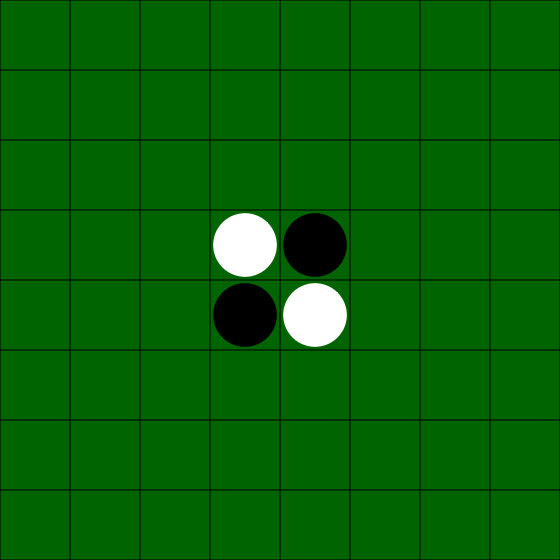
\includegraphics[width=\textwidth / 2]{board_initial}
    \caption{Initialer Spielzustand}
    \label{fig:board_initial}
\end{figure}

Zu Beginn des Spiels werden jeweils zwei Steine jedes Spielers so auf die vier mittleren Felder des Spielfelds gelegt, dass
– wie in Abbildung \ref{fig:board_initial} zu sehen – die Steine eines Spielers einander diagonal gegenüber liegen.

Die Spieler legen nun abwechselnd jeweils einen Stein ihrer eigenen Farbe auf das Spielfeld. Steine können nur auf freie
Felder gelegt werden, die in horizontale, vertikale oder diagonale Richtung an einen oder mehrere gegnerische Steine,
gefolgt von einem eigenen Stein, angrenzen. Eine beispielhafte Spielsituation, in der die möglichen Spielzüge für den
schwarzen Spieler als kleinere Kreise dargestellt werden, ist in \autoref{fig:board_possible_moves} zu sehen. 

\begin{figure}[H]
    \centering
    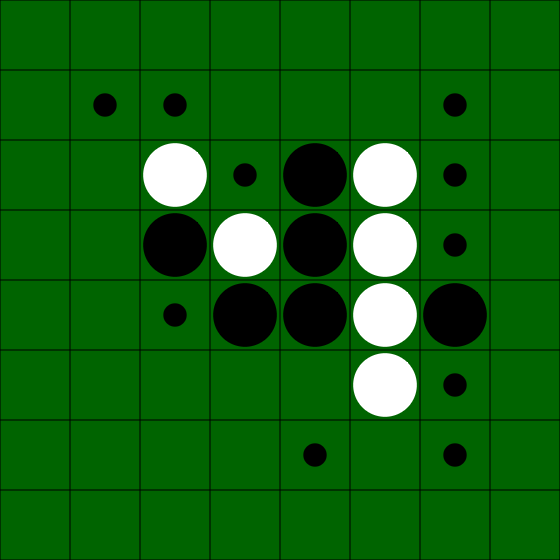
\includegraphics[width=\textwidth / 2]{board_possible_moves}
    \caption{Mögliche Züge des schwarzen Spielers}
    \label{fig:board_possible_moves}
\end{figure}

Alle gegnerischen Steine, die durch den gesetzten Stein in eine der 8 Richtungen lückenlos eingeschlossen werden, ohne dass sich freie Felder dazwischen befinden, werden umgedreht und erhalten dadurch die Farbe des Spielers, der diesen Zug ausgeführt hat.

Ist einer der Spieler zugunfähig, das heißt, er ist an der Reihe, kann jedoch keinen validen Zug spielen, so ist der
andere Spieler erneut am Zug.

Das Spiel endet, sobald beide Spieler zugunfähig sind. Der Gewinner ist dann der Spieler, der die meisten Steine seiner
Farbe auf dem Spielfeld liegen hat.
\cite{worldothellorules}


\section{Spieltheorie}
\label{sec:spieltheorie}

Eine mathematische Betrachtung von Spielen erfordert eine abstrakte Darstellung derselben. Ein Spiel kann dabei
verschiedene Eigenschaften haben. Auf das Spiel Othello treffen beispielsweise die folgenden Eigenschaften zu:

\begin{itemize}
    \item Determinismus
    \item Rundenbasiertheit
    \item Zwei-Spieler
    \item Nullsummenspiel
    \item Perfekte Information
\end{itemize}

Die Eigenschaft des Determinismus schließt auf Zufall basierende Elemente aus, die beispielsweise in Würfelspielen durch
das Würfeln einer zufälligen Zahl auftreten. Da in Othello jeder Spielzug nur von der Entscheidung des Spielers abhängt,
wird diese Eigenschaft erfüllt. Im Spielverlauf sind zudem immer zwei Spieler abwechselnd am Zug. Folglich werden auch
die Eigenschaften Zwei-Spieler und Rundenbasiertheit erfüllt. Bei einem Nullsummenspiel handelt es sich um ein
Spiel, bei dem das Ergebnis beider Spieler am Ende jedes Spiels die gleiche Summe hat. Beim Schach bekommt z. B. der
Gewinner einen Punkt und der Verlierer keinen Punkt, bei einem Unentschieden bekommen beide Spieler einen halben Punkt.
Die Summe beträgt also immer eins. Diese Regel kann auch in Othello angewandt werden, da ein Spiel entweder mit einem
Sieg und einer Niederlage oder einem Unentschieden endet. Um die Höhe des Sieges zu berücksichtigen, kann für jeden
Spieler die Anzahl der Steine gezählt werden. Dabei müssen lediglich nicht belegte Felder berücksichtigt und
beispielsweise für den Gewinner mit mehr Steinen gezählt werden. Da sich die Anzahl der Gesamtfelder nicht ändert,
beträgt die Summe der Punkte beider Spieler bei einer Spielfeldgröße von $8\times 8$ immer 64 und somit handelt es sich
bei Othello um ein Nullsummenspiel. Bei einem Spiel mit perfekter Information können beide Spieler zu jeder Zeit den
kompletten Zustand des Spiels einsehen. Anders als bei vielen Kartenspielen, in denen die Karten der
Gegenspieler unbekannt sind, ist das in Othello der Fall.
\cite[S.~161f.]{ai2010russel}

Formal besteht ein Spiel aus folgenden sechs Elementen:
\begin{enumerate}
    \item $S_0$ ist der Anfangszustand zu Beginn des Spiels.
    \item $Player(s)$ ist eine Funktion, die in einem Spielzustand $s$ den Spieler berechnet, der gerade an der Reihe
    ist.
    \item $Actions(s)$ ist eine Funktion, die für einen Spielzustand $s$ alle gültigen Züge berechnet.
    \item $Result(s, a)$ ist eine Funktion, die für einen Spielzustand $s$ und eine Aktion, also einen Spielzug $a$
    einen neuen Spielzustand berechnet.
    \item $TerminalTest(s)$ ist eine Funktion, die für einen Spielzustand $s$ berechnet, ob das Spiel vorbei ist oder
    nicht. Zustände, an denen das Spiel vorbei ist, werden Endzustände genannt.
    \item $Utility(s, p)$ ist eine Funktion, die für einen Endzustand $s$ ein numerisches Endergebnis für den Spieler
    $p$ berechnet.
\end{enumerate}


\section{Suchbäume}
\label{sec:gametree}

Ein Spiel kann als Baum dargestellt werden, dessen Wurzel gleich dem Startzustand des Spiels ist. Die Kanten des Baums
stellen Aktionen dar, die zu einem neuen Knoten, also einem neuen Spielzustand, führen. Vorerst sei angenommen, dass ein
bestimmter Spielzustand, in dem das Spiel gewonnen ist, gesucht wird und die Spielzüge des Gegners ausgesucht werden
können. Dieses Suchproblem hat als Lösung eine Abfolge von Aktionen, die zum Sieg des Spiels führen. Jeder Knoten kann
so erweitert werden, dass für jeden möglichen Spielzug, also jede Aktion, eine Kante zu einem neuen Knoten, also zu
einem neuen Spielzustand, führt. Der Baum kann dann nach einem bestimmten Zustand durchsucht werden, der das gegebene
Problem löst. Die Vorgehensweise dabei ist eine Tiefensuche. Zunächst wird eine Option bis zum Ende des Spiels
untersucht und erst wenn diese nicht zu einer Lösung des Problems führt, werden die übrigen Optionen in Betracht
gezogen.
\cite[S.~75]{ai2010russel}

\subsection{Adversative Suche}
In einem Spiel können die Züge des Gegners nicht beeinflusst werden. Deswegen ist ein einzelner Pfad von Aktionen
uninteressant und eine sogenannte Strategie, die für jeden Zug alle möglichen Reaktionen des Gegners betrachtet, ist
gesucht. Eine optimale Strategie führt unter der Annahme, dass auch der Gegner optimal spielt, zu einem mindestens
genauso guten Ergebnis wie jede andere Strategie.
\cite[S.~163f.]{ai2010russel}

Der Baum eines gesamten Spiels kann je nach Spiel sehr groß sein. Für das Spiel Othello besteht der Baum bei der Annahme
von einer durchschnittlichen Spiellänge von 58 Zügen und zehn Möglichkeiten pro Spielzug aus $10^{58}$ Knoten. Bei drei
verschiedenen Zuständen, die jedes Feld annehmen kann (frei, belegt von schwarz oder belegt von weiß), liegt die
Speicherkomplexität bei $3^{64}\approx10^{30}$ möglichen Spielzuständen. Diese Zahl lässt sich durch Ausschließen
offensichtlich ungültiger Zustände, in denen beispielsweise die mittleren vier Felder nicht belegt sind oder gesetzte
Steine nicht verbunden sind, auf ca. $10^{28}$ reduzieren \cite[S.~167]{searchingforsolutions}.
Bei einer Repräsentation von 2 Bit pro Feld, also 16 Byte pro Spielzustand, würden diese Zustände ca. $10^{20}$\,GB
Speicher benötigen. Der Spielbaum muss in diesem Fall also als theoretisches Konstrukt betrachtet werden, da er nicht
komplett dargestellt werden kann. Ein Suchbaum ist ein Teil des Spielbaums, der jedoch nur die für eine Entscheidung
relevanten Knoten beinhaltet.
\cite[S.~162f.]{ai2010russel}

Im allgemeinen Fall können Zustände mehrfach im Baum auftreten. Das passiert, wenn Spielzüge rückgängig gemacht werden
können. Beispielsweise können im Schach manche Figuren auf das vorherige Feld zurückgestellt werden. Für diese Spiele
ist es sinnvoll, zyklische Pfade auszuschließen. Dadurch wird verhindert, dass durch beliebig viele Wiederholungen eine
unendliche Menge an Pfaden entsteht.
\cite[S.~75]{ai2010russel}

In dem Spiel Othello kann allerdings kein Zustand mehrfach auftreten, da nach jedem Spielzug genau ein Spielstein mehr
auf dem Feld liegt und Spielsteine nicht wieder weggenommen werden können.


\section{Der Minimax-Algorithmus}

Minimax ist ein Algorithmus zur Bestimmung des optimalen Spielzugs in einem deterministischen, rundenbasierten, zwei-Spieler Nullsummenspiel mit perfekter Information.

Dabei wird für jeden Knoten im Spielbaum des Spiels, durch Rekursion, der Nutzen des entsprechenden Spielzustands für alle Spieler bestimmt.
An den Blatt-Knoten des Spielbaums ist der Nutzen für alle Spieler, in Form des Spielergebnisses, bereits bekannt.
Die Nutzen-Werte der restlichen Knoten werden bestimmt, indem, unter der Annahme das beide Spieler optimal spielen, immer der größte Nutzen aus den Kind-Knoten für den aktuell spielenden Spieler ausgewählt wird.
\cite[S.~165]{ai2010russel}

Dadurch lässt sich zu jedem Spielzustand der Zug bestimmen, der gegen einen optimal spielenden Gegner von größtem Nutzen ist.

Da bei einem zwei-Spieler Nullsummenspiel die Summe der Nutzen der beiden Spieler konstant ist, und sich somit der Nutzen für einem Spieler aus dem Nutzen des anderen Spielers ergibt, muss nur der Nutzen für einen Spieler betrachtet werden. Dieser wird dann abwechselnd von diesem Spieler maximiert, und von dessen Gegner minimiert.
Die Spieler werden dann maximierender und einen minimierender Spieler genannt.
Aus diesem Vorgehensweise ergibt sich der Name "'Minimax"' für die zwei-Spieler Variante des Algorithmus.
Bei Spielen mit mehr als zwei Spielern kann diese Optimierung nicht angewandt werden, weshalb in diesem Fall immer der Nutzen für alle Spieler getrennt betrachtet werden muss.
\cite[S.~165]{ai2010russel}

%TODO: Mathematische Beschreibung / evtl. Implementation





\section{Heuristische Evaluations-Funktion}

In vielen relevanten Spielen ist es aufgrund der Größe des Suchbaums praktisch nicht möglich diesen vollständing zu
durchsuchen. In der Praxis kann der Suchbaum deshalb nur bis zu einer begrenzten Tiefe durchsucht werden. An diesem
Punkt kommt eine heuristische Evaluations-Funktion zum Einsatz, welche den Nutzen des Spielzustands für einen Spieler
approximiert.
\cite[S.~171]{ai2010russel}

Optimalerweise würde die Evaluations-Funktion den tatsächlichen Nutzen einer Spielsituation bestimmen. Eine solche
Evaluations-Funktion ist durch den Minimax Algorithmus gegeben. Aus offensichtlichen Gründen, kann diese jedoch nicht
zum Einsatz kommen, da der Rechenaufwand hierbei identisch zu einer vollständigen Suche wäre.

Um den Nutzen verschiedener Spielzüge miteinander zu vergleichen, wird also eine weniger rechenaufwändige
Evaluations-Funktion benötigt, die diesen nur ausreichend gut annähert, statt den tatsächlichen Nutzen zu bestimmen.

Durch die Anwendung einer approximierten Evaluations-Funktion verliert der Minimax Algorithmus seine Optimalität. Es
wird also nichtmehr garantiert der Zug mit dem größten Nutzen gewählt. Mit einer passend gewählten Evaluations-Funkion
können dennoch gute Ergebnisse erzielt werden, die in vielen Spielen die Fähigkeiten eines menschlichen Gegenspielers
übertreffen. Die Spielstärke der KI wächst mit zunehmender Suchtiefe.

Ein primitiver Ansatz für eine Evaluations-Funktion bei dem Spiel Othello ist die Differenz der Anzahlen von eigenen
Steinen und gegnerischen Steinen auf dem Spielfeld, da diese am Ende über den Sieg entscheidet. Gegen Ende eines Spiels
könnte dieser Ansatz eine passende Bewertung liefern, allerdings kann es vor allem in der Anfangsphase sinnvoll sein,
weniger Steine zu haben. Viel wichtiger ist z.\,B. die Möglichkeit, neue Steine zu platzieren.

Diesen Ansatz verfolgt die Betrachtung der Mobilität.

Die aktuelle Mobilität ist ein Maß dafür, wie viele mögliche Züge die Spieler haben. Eine niedrige Anzahl an möglichen
Zügen ist häufig schlecht, da der Spieler gezwungen ist, einen weniger guten Zug zu machen. Als quantitatives Merkmal
kann zunächst die Differenz der möglichen Züge beider Spieler betrachtet werden. Allerdings ist eine Stellung häufig
besser, wenn man mehr mögliche Züge hat und der Gegner bei gleicher Differenz weniger mögliche Züge hat. Um diese
Tatsache zu berücksichtigen, kann eine nicht-lineare Funktion verwendet werden.
%TODO: Buro verwendet aus Performancegründen eine Approximation
\cite[S. 7]{evaluationfunctions}

Neben der aktuellen Mobilität kann auch die potenzielle Mobilität betrachtet werden. Diese ist ein Indikator für die
mögliche Mobilität in folgenden Zügen. Michael Buro hat als aussagekräftigstes Merkmal die Summe aller Anzahlen freier
Felder um gegnerische Steine ausgemacht.
\cite[S. 8f.]{evaluationfunctions}


\section{Alpha-Beta-Pruning}

Die Alpha-Beta-Pruning ist eine Optimierung des Minimax Algorithmus, bei der komplette Zweige des Suchbaums ausgeschlossen werden können, die das Ergebnis des Algorithmus' nicht mehr beeinflussen können.
Ein Zweig kann ausgeschlossen werden, wenn für einen Spieler bereits ein Zug mit einem größeren Nutzen gefunden wurde, als bei dem zu betrachtenden Zweig maximal noch erzielbar ist.

Durch Anwendung von Alpha-Beta-Pruning wird das Ergenis des Minimax Algorithmus' nicht beeinflusst. Jeoch kann durch die Betrachtung einer geringeren Zahl von Knoten die Performanz signifikant verbessert werden.

Bei einer nicht vollständingen Alpha-Beta-Suche, unter Anwendung einer heuristischen Evaluations-Funktion kann gegenüber dem Minimax Algorithmus die maximale Suchtiefe bei gleicher Rechenzeit erhöht werden, was zu einem besseren Ergebnis führt.

Da Alpha-Beta-Pruning nur dann Zweige ausschließen kann, wenn bereits bessere Zweige betrachtet wurden ist es von Vorteil, die Zweige in der Reihenfolge absteigenden Nutzens zu betrachten, da so die Anzahl der ausgeschlossenen
Zweige maximiert werden kann.
Dies ist jedoch in der Praxis nicht optimal möglich, da dafür ja bereits eine korrekte Bewertung der Züge stattgefunden haben muss, was die Anwendung der Alpha-Beta Suche überflüssig machet.
Eine ungefähre Anordnung der Züge, die dennoch zu einer wesentlichen Effizienzverbesserung führt ist jedoch häufig möglich. Beispielsweise können beim Schach Züge in denen eine gegnerische Figur
geschlagen wird priorisiert werden, und beim Othello Züge in den Ecken und am Rand des Spielfelds, gegenüber denen in der Mitte bevorzugt werden.

\section{ProbCut}

Der Minimax-Algorithmus erfordert in seiner Grundform das Durchsuchen des kompletten Spielbaums.
Die Optimierung des Alorithmus durch die Alpha-Beta-Suche ermöglicht zwar das Weglassen von Teilen des Spielbaums, aber da auch hier der korrekte Minimax-Wert berechnet werden muss, kann der Baum nur rückwärts reduziert werden.

ProbCut erweitert die Alpha-Beta-Suche durch eine statistische Betrachtung, wobei auch Zweige, die nur mit einer bestimmten Wahrscheinlichkeit nicht zu einer Veränderung des Ergebnisses beitragen, weggelassen werden können.
Die mithilfe von ProbCut durchgeführten Verkleinerungen des Baums werden "`probabilistic forward cuts"' genannt.

Ein Zug ist dann für die Entscheidung irrelevant, wenn dessen Minimax Wert außerhalb des Alpha-Beta Fensters, dh. außerhalb des Intervalls \([\alpha,\beta]\) liegt, da dieser Zug von beiden Spielern umgangen wird und deshalb im Spiel nicht auftritt.
Dies entspricht der Abbruchbedingung beim Alpha-Beta Algorithmus.
Ob das der Fall ist ist jedoch in der Regel erst nach Anwendung des Alpha-Beta Algorithmus' mit der maximal gewünschten Suchtiefe bekannt.

ProbCut stellt einen statistischen Zusammenhang zwischen dem Minimax Wert einer tieferen Suche der Tiefe \(d\) und dem Wert einer flacheren Suche der Tiefe \(d'<d\) her.
Anhand des Minimax Werts der flachen Suche wird bestimmt ob der Wert der tiefen Suche mit einer gegebenen Wahrscheinlichkeit \(p\) außerhalb des Alpha-Beta Fensters liegt.
Ist dies der Fall so wird bereits nach der flachen Suche abgebrochen, sodass die Tiefe Suche nicht mehr durchgeführt werden muss.

Dazu verwendet ProbCut ein lineares statistisches Modell \(v=a*v'+b+e\) wobei \(v\) der Minimax Wert der tiefen Suche, \(v'\) der Minimax Wert der flachen Suche, \(a\) und \(b\) konstanten und \(e\) eine normalverteilte Fehlervariable ist.
\(a\) und \(b\) werden im Vorraus so gewählt dass die Standardabweichung \(\sigma\) von \(e\) möglichst gering ist.

Daraus lässt sich herleiten dass mit einer Wahrscheinlichkeit von mindestens \(p\) gilt:

\(v<=\alpha\) genau dann wenn \(v'<=(\Phi^{-1}(p)*\sigma+\alpha-b)/a\)

und

\(v>=\beta\) genau dann wenn \(v'>=(-\Phi^{-1}(p)*\sigma+\beta-b)/a\)

Trifft nach der flachen Suche einer der beiden Fälle auf der rechten Seite ein, so wird keine tiefe Suche durchgeführt, da \(v\) nach der linken Seite min Wahrscheinlichkeit \(p\) ausßerhalb des Alpha-Beta Fensters liegt
und somit nicht relevant ist.

Wie auch beim Alpha-Beta Algorithmus ergibt sich der Vorteil von ProbCut durch die Zeitersparnis, die durch das Weglassen von Zweigen erreicht wird. Dadurch kann die Suchtiefe bei den relevanten Zweigen erhöht werden.
\cite[S.~1]{probcut}



	\clearpage

	% Literaturverzeichnis
	\cleardoublepage
	\printbibliography

	% Glossar
	\printglossary[style=altlist,title=\langglossar]
	
	% sonstiger Anhang
	%\clearpage
	%\appendix
	%% !TeX root = ../dokumentation.tex

\addchap{\langanhang}

\section*{A. Gewichtung der aktuellen und potenziellen Mobilität}
 
\setcounter{table}{0}
\renewcommand{\thetable}{A\arabic{table}}

\begin{table}[hb]
\centering
\begin{tabular}{c|c|ccc}
\hline
Heuristik S\,/\,W & \#Spiele & Siege S & Unentschieden & Siege W \\
\hline
 A\,/\,B & 20 & 50\,\% &  2\,\% & 48\,\% \\
 A\,/\,C & 20 & 46\,\% &  4\,\% & 50\,\% \\
 A\,/\,D & 20 & 32\,\% &  8\,\% & 60\,\% \\
 B\,/\,C & 20 & 48\,\% &  2\,\% & 50\,\% \\
 B\,/\,D & 20 & 42\,\% &  2\,\% & 56\,\% \\
 C\,/\,D & 20 & 40\,\% &  2\,\% & 58\,\% \\
\hline
\end{tabular}
\caption{Einfluss aktueller und potenzieller Mobilität auf den Anteil der Siege}
\label{table:mobility}
\end{table}

\small{
A: Nur aktuelle Mobilität \\
B: Nur potenzielle Mobilität \\
C: Wechsel von potenzieller zu aktueller Mobilität bei 36 Steinen auf dem Spielfeld \\
D: Lineare Kombination von potenzieller und aktueller Mobilität}

\pagebreak

\section*{B. Anzahl der Steine als Heuristik am Ende des Spiels}
 
\setcounter{table}{0}
\renewcommand{\thetable}{B\arabic{table}}

\begin{table}[hb]
\centering
\begin{tabular}{c|c|ccc}
\hline
Verwendete Heuristik S\,/\,W & \#Spiele & Siege S & Unentschieden & Siege W \\
\hline
 A\,/\,B & 20 &100\,\% &  0\,\% & 0\,\% \\
 A\,/\,C & 20 & 90\,\% & 10\,\% & 0\,\% \\
\hline
\end{tabular}
\caption{Einfluss der Anzahl der Steine auf den Anteil der Siege}
\label{table:disccount}
\end{table}

\small{
A: Heuristik ohne Anzahl der Steine (Mobilität und Cowtello) \\
B: Anzahl der Steine ab 50 belegten Feldern \\
C: Anzahl der Steine ab 58 belegten Feldern}

\pagebreak
%\includepdf[pages=-,scale=.9,pagecommand={}]{Aufgabenstellung.pdf} % PDF um 10% verkleinert einbinden --> Kopf- und Fußzeile  werden so korrekt dargestellt. Die Option `pages' ermöglicht es, eine bestimmte Sequenz von Seiten (z.B. 2-10 oder `-' für alle Seiten) auszuwählen.


	
\end{document}
